\documentclass[portuguese,12pt,a4paper]{article}
\usepackage[T1]{fontenc}
\usepackage{float}
\usepackage{times}
\usepackage{graphicx}
\usepackage[portuguese]{babel}
\usepackage{titlesec}
\usepackage{amsbsy}
\usepackage[table,xcdraw]{xcolor}
\usepackage{multirow}
\usepackage{adjustbox}
\usepackage{fancyhdr}
\usepackage{indentfirst}
\usepackage[
top=2.5cm,
bottom=2.5cm,
right=3cm,
left=3cm]{geometry}
\renewcommand{\baselinestretch}{1.5} 
% Turn on the style
\fancypagestyle{mystyle}{
	\fancyhf{}
	\renewcommand\headrulewidth{0pt}
	\fancyfoot[R]{\thepage}
}

%Renew plain style for chapter pages
\fancypagestyle{plain}{
	\fancyhf{}
	\renewcommand\headrulewidth{0pt}
	\fancyfoot[R]{\thepage}
}
\setlength{\parindent}{1cm}

\usepackage[abnt-etal-text=it,abnt-and-type=& ]{abntex2cite}
\usepackage{pdfpages}
\addto\captionsportuguese{\renewcommand{\refname}{\normalsize   \ \ \ \ \ \ \ \ \ REFERÊNCIAS BIBLIOGRÁFICAS}}
\renewcommand{\refname}{REFERÊNCIAS BIBLIOGRÁFICAS }
\begin{document} 

	
\pagenumbering{roman}
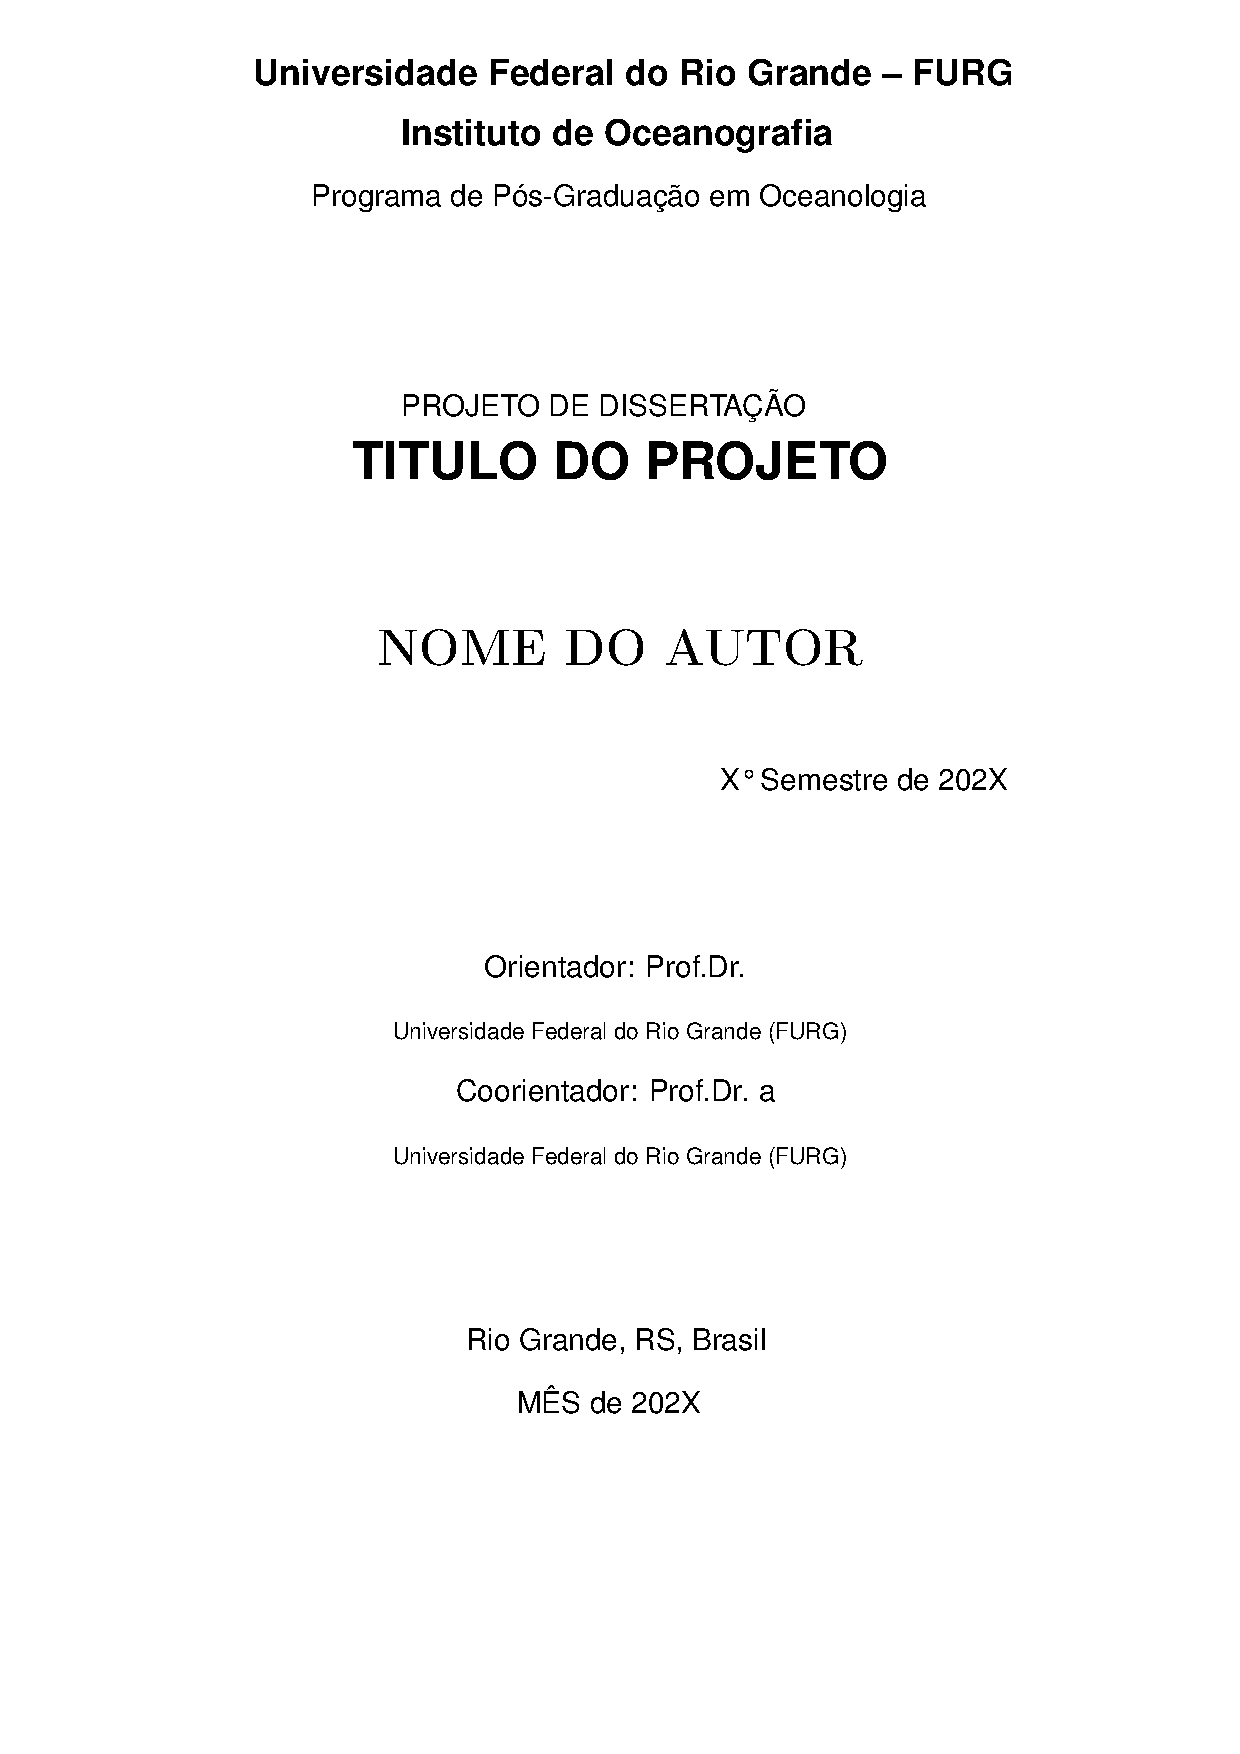
\includepdf[pages={1}]{../capa.pdf}
\newpage
\pagenumbering{arabic}
\textbf{RESUMO}\\

Os oceanos estão constantemente recebendo e dissipando energia, principalmente via
movimentos turbulentos. Uma boa parte dessa energia é recebida quando da atuação
do estresse do vento na superfície livre do mar o que, juntamente com a forçante
termohalina, impulsiona a circulação global dos oceanos, responsável pelo transporte
de propriedades físicas por todo o globo e sendo essencial para a vida e o clima. A
variabilidade sazonal dos campos de vento afeta a intensidade dessas correntes,
podendo gerar instabilidades e criar estruturas de mesoescala. A Corrente do Brasil é
uma Corrente de Contorno Oeste que faz parte do Giro Subtropical do Atlântico Sul,
nascendo de uma bifurcação da Corrente Sul Equatorial Sul numa latitude abaixo dos
12°S, sendo uma corrente gerada pela atuação dos ventos no oceano e,
consequentemente, sendo afetada pela sazonalidade destes ventos. Estudos sobre
como a energia cinética turbulenta varia sazonalmente são escassos no hemisfério Sul,
embora seja um assunto de interesse no hemisfério Norte. Partindo disso, esse
trabalho pretende estudar a variabilidade da energia cinética turbulenta associada à
Corrente do Brasil na região entre 20°S e 35°S, assim como estudar os processos
dinâmicos associados com esta variabilidade e também como o vento se relaciona com
ela. Esse trabalho irá utilizar dados do OFES e resolver os termos
energéticos pelo Diagrama de Lorenz. Esse trabalho abrange um tema de interesse
atual ainda não abordado com a Corrente do Brasil.\\

\textbf{INTRODUÇÃO} \\

Os oceanos estão em movimento de forma contínua, seja em movimentos a níveis
moleculares até as grandes correntes que regulam a circulação global, onde esse
movimento é causado pela energia recebida do Sol e é influenciado pela rotação da
Terra. A principal forma que essa energia recebida move os oceanos é através dos
ventos, que transferem energia para a superfície do oceano por fricção. O estresse
aplicado pelo vento na superfície é o suficiente para manter o espectro da energia
cinética (EC) no oceano em equilíbrio nas camadas superficiais [\citeauthoronline{ferrari2009ocean} \citeyear{ferrari2009ocean}]. A energia cinética embora seja a que tenha mais atenção, pela sua ligação fundamental com a dinâmica dos oceanos, não é a única forma com que a energia está disponível. Escoamentos possuem energia interna e potencial além da cinética [\citeauthoronline{vallis2006atmospheric} \citeyear{vallis2006atmospheric}], mas considerando um fluido de Boussinesq (uma boa aproximação para os oceanos), as conversões energéticas irão envolver apenas a energia potencial e cinética.

Dessa forma, a energia cinética oriunda da energia recebida pelo vento é a principal
responsável pela circulação dos oceanos e pela geração de turbulência, porém, a
maior parte dessa energia é consumida nesta geração próxima a superfície, 
não atingindo grandes profundidades do oceano. Parte da energia associada ao trabalho do vento é
levada às Correntes de Contorno Oeste (CCOs) e dissipada por elas, sendo uma boa
parte da energia removida por instabilidades baroclínicas [\citeauthoronline{wunsch2004vertical} \citeyear{wunsch2004vertical}]. A
energia potencial (EP), por sua vez, é relacionada com a distribuição do campo de
massa do fluido sendo a energia potencial disponível (EPD) aquela que participa nas
trocas energética dos oceanos. O conceito de EPD pode ser entendido como a energia
acumulada na coluna d’água estratificada em que as isopicnais possuem uma
determinada inclinação e onde o centro de massa da coluna encontra-se mais elevado
do que na situação em que as isopicnais se encontram alinhadas horizontalmente
(estado de referência) e onde a EPD é nula [\citeauthoronline{cushman2011introduction} \citeyear{cushman2011introduction}]. 

As CCOs geram um grande interesse do ponto de vista da energia cinética, como se
pode observar na Figura \ref{fig:ke}, onde as regiões com maior EC correspondem às regiões dominadas pelas CCOs, tais como as Corrente do Golfo, das Agulhas, Leste da Austrália, de Kuroshio e do Brasil. \citeauthoronline{ferrari2009ocean} (\citeyear{ferrari2009ocean}) sugerem que a EC nos oceanos tropicais é governada por variações sazonais devido a resposta das correntes equatoriais aos padrões do vento. As CCOs apresentam a formação de diversas estruturas de mesoescala, o que acontece tendo em vista que a reserva de EP devido a estratificação do escoamento é propícia à geração de instabilidade baroclínicas. A presença de instabilidades baroclínicas e barotrópicas possibilita a geração de vórtices que, por consequência, propiciam uma mistura vertical de momentum [\citeauthoronline{cushman2011introduction}, \citeyear{cushman2011introduction}].


\begin{figure}[H]
	\centering
	\includegraphics[width=0.9\linewidth]{ke}
	\caption{Estimativa da energia cinética geostrófica (cm/s$^2$) na superfície dos oceanos, multiplicada por $\sin^2\varphi$ (sendo $\varphi$ a latitude) para evitar erros nas regiões equatoriais [Fonte: \citeauthoronline{ferrari2009ocean}, \citeyear{ferrari2009ocean}]}
	\label{fig:ke}
\end{figure}


A Corrente do Brasil (CB) é uma Corrente de Contorno Oeste que transporta água quente e salina para as altas latitudes, sendo relativamente fraca em comparação a outras CCOs. Ela é mais rasa, fluindo entre a superfície e 700m de profundidade, sendo altamente baroclínica. A CB é formada em aproximadamente 10°S por uma bifurcação da Corrente Sul Equatorial (CSE), que gera a CB para sul e a Corrente Norte do Brasil para norte, possuindo um transporte que varia de ~4 Sv na sua formação até ~20 Sv na região próximo de seu encontro com a Corrente das Malvinas, onde forma a Confluência Brasil-Malvinas. Uma explicação para a CB ser relativamente mais fraca, surge no fato que a componente da circulação termohalina ter sentido oposto àquela da circulação gerada pelo vento [e.g., \citeauthoronline{silveira2000corrente}, \citeyear{silveira2000corrente}].

A CSE e, por consequência, a formação da CB, é afetada pela variabilidade sazonal da
posição da Zona de Convergência Intertropical (ZCIT) [\citeauthoronline{rodrigues2007seasonal}, \citeyear{rodrigues2007seasonal}]. Tal comportamento ocasiona um decaimento do transporte da CB em junho e julho e o seu consequente aumento entre setembro e novembro. Essa variação pode ser observada
na posição da Confluência Brasil-Malvinas que também está sujeita a uma variabilidade
sazonal [e.g \citeauthoronline{de2019driving}, \citeyear{de2019driving}]. Cabe destacar que tal sazonalidade pode interferir no clima da região.

Estudos sobre a sazonalidade da Energia Cinética Turbulenta (ECT) relacionada com CCOs praticamente só são encontrados com aplicação no hemisfério Norte, com uma exceção para a Corrente Leste da Austrália, que foi estudada recentemente em \citeauthoronline{liu2022} (\citeyear{liu2022}). As Correntes do Golfo e de Kuroshio receberam uma grande quantidade de trabalhos dedicados ao estudo da ECT de forma geral e sua sazonabilidade. \citeauthoronline{kang2016seasonal} (\citeyear{kang2016seasonal}) estudaram a variabilidade da ECT na Corrente do Golfo utilizando diversas simulações do ROMS, com durações aproximadas de 10 anos, onde foi observado que a conversão barotrópica tinha um pico durante o verão boreal, enquanto a conversão baroclínica tinha um pico no fim do inverno boreal e começo da primavera, sendo a sazonalidade do vento um fator crucial nessa mudança. \citeauthoronline{yang2017decadal} (\citeyear{yang2017decadal}) estudaram a variabilidade decadal da ECT associada à Corrente de Kuroshio em toda a sua extensão, utilizando dados do ECCO entre 1993 a 2015, quando foi observado que a instabilidade barotrópica é a principal fonte da variação decadal e dos meandramentos responsáveis pela geração da ECT na direção norte da corrente. Neste trabalho se levanta a hipótese da variabilidade do vento estar causando a instabilidade barotrópica devido a propagação de ondas de Rossby baroclínicas.

A interação entre a energética e a sua variabilidade sazonal aplicada a uma CCO ainda não é totalmente entendida [e.g \citeauthoronline{kang2016seasonal}, 2016]. A hipótese levantada por \citeauthoronline{ferrari2009ocean} (\citeyear{ferrari2009ocean}) sobre a forma que a variabilidade do vento afeta as correntes em oceanos tropicais carece de estudos do ponto de vista energético. Na CB os estudos sobre a influência das variações sazonais nos termos energéticos ao longo da coluna da água são escassos. Estudos energéticos sobre a CB, com a utilização do Diagrama de Lorenz, foram desenvolvidos em \citeauthoronline{Brum-2017} (\citeyear{Brum-2017}) e \citeauthoronline{magalhaes2017energetics} (\citeyear{magalhaes2017energetics}).

Este Projeto de Mestrado visa preencher esta lacuna do conhecimento de como a
energética associada com a CB se relaciona com a sua variabilidade sazonal, com
destaque para os principais processos dinâmicos que influenciam a energética
analisada, assim como também será dado destaque para a influência do vento local em
tal variabilidade.
 \\


\textbf{JUSTIFICATIVA E RELEVÂNCIA } \\

Conhecer como a energética de uma região que é percorrida por uma CCO se comporta em cada etapa do
ano é de extrema importância para o entendimento de toda a dinâmica da
mesma. Diante disso, alguns estudos recentes (e.g. \citeauthoronline{kang2016seasonal}, \citeyear{kang2016seasonal}; \citeauthoronline{zhang2021seasonal}, \citeyear{zhang2021seasonal}; \citeauthoronline{liu2022},  \citeyear{liu2022}; \citeauthoronline{yan2023seasonal}, \citeyear{yan2023seasonal}) têm
buscado estudar a sazonalidade da ECT em Correntes de Contorno Oeste.
Aplicar tal estudo na Corrente do Brasil, a CCO da costa brasileira, é
importante para um melhor entendimento dos principais processos dinâmicos
que afetam a variabilidade sazonal desta corrente estendendo-se ainda tal estudo para a influência do vento nesta energética. \\

\textbf{OBJETIVO GERAL} \\ 

Esta proposta de trabalho tem como objetivo geral estudar a variabilidade sazonal da Energia Cinética Turbulenta associada com a Corrente do Brasil entre 20°S e 35°S. \\

\textbf{OBJETIVOS ESPECÍFICOS} 

\begin{itemize}
\item  Associar a variabilidade sazonal da ECT em cada subdomínio de estudo com os
respectivos processos dinâmicos associados,

\item  Relacionar o trabalho do vento sobre a superfície livre do mar com a variabilidade sazonal da ECT,

\item Adaptar/avaliar o pacote Lorenz Energy Cycle – LEC para a sua utilização com as saídas numéricas do modelo numérico OFES, tornando-o apto a trabalhar com
saídas tanto do HYCOM (status atual do pacote) como do OFES. 
\end{itemize}

\textbf{MATERIAL E MÉTODOS} \\

Nessa seção serão apresentados os dados a serem utilizados, a divisão da região de
estudo e, por fim, a forma pela qual se pretende calcular os termos energéticos seguida pela análise dos resultados. \\

\textbf{Saídas Numéricas}

As saídas numéricas do modelo OFES serão utilizadas no presente trabalho. Este modelo resolve as equações primitivas para o oceano com uma resolução da sua grade numérica de 1/10° com 54 níveis verticais. A topografia do modelo é construída a partir da base de dados do OCCAM com resolução de 1/30°  [\citeauthoronline{masumoto2004fifty}, \citeyear{masumoto2004fifty}]. A resolução do modelo OFES permite que ele consiga resolver completamente os sinais de mesoescala, os quais são do interesse desse trabalho. O OFES é um modelo que vem sendo cada vez mais utilizado para estudos que
envolvem análises energéticas  [e.g. \citeauthoronline{zhang2021seasonal}, \citeyear{zhang2021seasonal} e \citeauthoronline{yan2023seasonal}, \citeyear{yan2023seasonal}]. Este modelo oferece uma vantagem sobre outros modelos numéricos na questão da análise energética pois ele disponibiliza as componentes zonal e meridional do estresse do vento. As saídas numéricas para a região de estudo, conforme mostra a Figura \ref{fig:area}a, serão obtidas no site \url{https://www.jamstec.go.jp/ofes/ofes.html}. \\


\textbf{Divisão da Região de Estudo}

Previamente, o campo médio do escoamento da CB foi obtido para toda a região de estudo (20°S até 35°S). De acordo com este campo, a região foi posteriormente dividida em três subdomínios menores, com características batimétricas/topográficas marcantes em cada um deles (ver a Figura \ref{fig:area}a) que
influenciam a CB e os seus respectivos campos energéticos. A área de estudo foi
separada então em três subdomínios onde a variabilidade sazonal da CB será
analisada, conforme ilustrado na Figura \ref{fig:area}b.

\begin{figure}[H]
	\centering
	\includegraphics[width=1.01\linewidth]{area}
	\caption{Região de estudo. (a) Batimetria da região de estudo mostrando as regiões de interesse para a divisão dos subdomínios (Cabo Frio, RJ; Santos,SP e o Cone de Rio Grande) juntamente com as isóbatas de 200m,1000m e 2000m. (b) Campo médio de velocidade da Corrente do Brasil com a respectiva área de cada subdomínio, em vermelho o subdomínio de Cabo Frio, em amarelo o subdomínio da Bacia de Santos e em verde o subdomínio do Cone de Rio Grande.}
	\label{fig:area}
\end{figure}

No subdomínio norte, na região de Cabo Frio, onde há uma brusca alteração da linha
de costa, a CB apresenta um comportamento que permite a formação de diversos sistemas de meandramentos e formação de vórtices [e.g. \citeauthoronline{mano2009energy}, \citeyear{mano2009energy}]. O
segundo subdomínio, na região da Bacia de Santos, apresenta isóbatas que norteiam o
escoamento da CB numa orientação aproximadamente constante, na direção nordeste-
sudoeste. No subdomínio sul é destacada a presença de uma dorsal oceânica
chamada de Cone de Rio Grande que afeta o comportamento energético da CB na
região [\citeauthoronline{Brum-2017}, \citeyear{Brum-2017}]\\

\textbf{Cálculo dos Termos Energéticos}

O pacote  \textit{Lorenz Energy Cycle - LEC}, desenvolvido no LEOC para a linguagem de programação Octave, de autoria de \citeauthoronline{pacotelec} (\citeyear{pacotelec}), que utiliza o Diagrama de Lorenz na obtenção dos termos energéticos, será utilizado
para a realização dos cálculos dos termos energéticos. O Pacote LEC foi desenvolvido inicialmente para o modelo numérico HYCOM, e será adaptado no presente estudo para o modelo OFES. O Diagrama de Lorenz esquematiza as trocas energéticas entre os reservatórios de energia cinética e potencial no oceano (em suas formas média e turbulenta), disponibilizando formas de quantificar os diversos termos que compõem quatro balanços de energia (ECM,ECT,EPM,EPT) e também as trocas entre diferentes compartimentos energéticos, tais como a energia entregue pelo vento ao oceano. A energia potencial será tratada na sua forma disponível para conversões energéticas, onde o conceito de energia potencial disponível e ciclo de energia foram primeiro introduzidos em \citeauthoronline{margules1903uberdie} (\citeyear{margules1903uberdie}), tendo sido amplamente utilizados desde então. A Figura \ref{fig:diagrama} mostra uma forma atual do Diagrama de Lorenz.

\begin{figure}[H]
	\centering
	\includegraphics[width=0.6\linewidth]{diagrama}
	\caption{Diagrama de Lorenz mostrando a relação entre os reservatórios de energia, sendo ECM a energia cinética media, ECT a energia cinética turbulenta, EPM a energia potencial média e EPT a energia potencial turbulenta. [Fonte: \citeauthoronline{magalhaes2017interaccao}, \citeyear{magalhaes2017interaccao}] }
	\label{fig:diagrama}
\end{figure}

Inicialmente, para a realização de uma análise sazonal dos termos energéticos (com ênfase principal na ECM e ECT), estes serão calculados na forma de médias climatológicas mensais para um intervalo temporal de 2000 a 2014. Médias mensais por estação também serão contempladas para efeito de análise das variações sazonais dos termos energéticos (anomalias, etc). As expressões energéticas que serão utilizadas, a princípio no presente trabalho são [e.g \citeauthoronline{azevedo2008processos}, \citeyear{azevedo2008processos} e \citeauthoronline{Brum-2017}, \citeyear{Brum-2017}]:

\begin{equation}
ECT = \rho_0 \frac{1}{2} \overline{(u'^2 + v'^2)}
\end{equation}
\begin{equation}
	ECM = \rho_0 \frac{1}{2} [(\overline{u})^2 +  (\overline{v})^2]
\end{equation} 
\begin{equation}
CBT = - \rho_0 \Big[\overline{u'u'}\frac{\partial\overline{u}}{\partial x}  +  \overline{u'v'}\Big(\frac{\partial\overline{u}}{\partial y} +\frac{\partial\overline{v}}{\partial x} \Big) +  \overline{v'v'}\frac{\partial \overline{v}}{\partial y} \Big]
\end{equation}
\begin{equation}
	CBC = -\frac{g^2}{\rho_0 N^2}\overline{\boldsymbol{u}_h'\rho'}\cdot\nabla_h\overline{\rho}
\end{equation}
\begin{equation}
FDTV  = -g\overline{w'\rho'}
\end{equation}  sendo $u$, $v$ e $w$ as componentes zonais, meridionais e vertical, respectivamente, da velocidade da CB [m/s], $\overline{()}$ a media climatológica  e $()'$ o desvio dessa média, $\rho$ a densidade [kg/m$^3$], $\rho_0$ a constante para a densidade da água do mar [1025 kg/m$^3$], $\boldsymbol{u}_h$ é a velocidade horizontal [m/s], $\nabla_h$ o operador nabla horizontal e $g$ a gravidade [m/s$^2$]. Variáveis em negrito são vetoriais. Os termos CBT e CBC representam a taxa de conversão da ECT devido à instabilidade barotrópica e baroclínica, respectivamente. O termo FDTV representa o fluxo de densidade turbulento vertical, sendo um termo fundamental para entender como a instabilidade baroclínica se relaciona com a ECT, conforme a Figura \ref{fig:diagrama}.

A forçante do vento, que influencia o campo turbulento e sua própria variabilidade, deverá, a princípio, afetar a sazonalidade da energia cinética associada com a CB. Os termos turbulentos e médio do trabalho realizado pelo vento sobre a superfície livre do mar, nos campos turbulento e médio, podem ser estimados diretamente, seguindo-se \citeauthoronline{yan2023seasonal} (\citeyear{yan2023seasonal}), pelas expressões para o Trabalho do Vento Turbulento (TVT) e Trabalho do Vento Médio (TVM):
\begin{equation}\label{eww}
TVT = \overline{\boldsymbol{V}'\cdot \boldsymbol{\tau'}}
\end{equation} onde $\boldsymbol{\tau}$ é o estresse do vento na superfície [N/m$^2$] e $\boldsymbol{V}$ representa o vetor velocidade do vento. 
Para o campo médio, a equação \ref{eww} toma a forma:
\begin{equation}
TVM = \overline{\boldsymbol{V}'} \cdot \overline{\boldsymbol{\tau^{\textcolor{white}{.}}}}
\end{equation} 


\textbf{Análises dos Resultados}

Com o cálculo dos termos energéticos espera-se identificar os principais processos dinâmicos, do ponto de vista sazonal, associados com a energética da CB e também a importância da atuação do vento nesta energética. Ferramentas de análise estatística e outras serão definidas no transcorrer do estudo aqui desenvolvido para um melhor andamento do trabalho na sua parte final.
Ao final do estudo, um artigo será submetido a um periódico internacional, seguindo-se as normas do PPGO, onde a variabilidade dos termos energéticos associados com a CB na região de estudo será analisada e discutida.\\

\textbf{VIABILIDADE} \\ 

Esse trabalho será realizado nas dependências do CEOCEAN, no Laboratório de
Estudos dos Oceano e Clima - LEOC, onde está disponível a capacidade de
processamento necessária para o processamento do grande volume de dados
relacionados com a execução deste trabalho (com a utilização de workstations). \\

\textbf{CONTRIBUIÇÃO CIENTÍFICA} \\

O estudo da variabilidade sazonal da energética aplicado à Corrente do Brasil com a
utilização do Diagrama de Lorenz ainda não foi realizado pela comunidade científica,
sendo um assunto de interesse atual no hemisfério Norte. Os resultados desse estudo
serão extremamente importantes para um melhor entendimento da energética da CB. \\

\textbf{CRONOGRAMA} \\

O cronograma de atividades proposto para a realização do presente trabalho é
apresentado na Tabela 1. 
\begin{table}[H]

	\centering

	\begin{adjustbox}{width=1\textwidth}

	\begin{tabular}{|l|cccc|ccccc|c|}
		\hline
		ANO                            & \multicolumn{4}{c|}{2023}                                                                                                                                                & \multicolumn{5}{c|}{2024}                                                                                                                                                                                 & 2025                  \\ \hline
		BIMESTRE                       & \multicolumn{1}{c|}{}                          & \multicolumn{1}{c|}{}                          & \multicolumn{1}{c|}{}                          &                       & \multicolumn{1}{c|}{}                      & \multicolumn{1}{c|}{}                      & \multicolumn{1}{c|}{}                      & \multicolumn{1}{c|}{}                      &                       &                       \\ \cline{1-1}
		ATIVIDADES                     & \multicolumn{1}{c|}{\multirow{-2}{*}{M-A}}     & \multicolumn{1}{c|}{\multirow{-2}{*}{M-J}}     & \multicolumn{1}{c|}{\multirow{-2}{*}{S-O}}     & \multirow{-2}{*}{N-D} & \multicolumn{1}{c|}{\multirow{-2}{*}{J-F}} & \multicolumn{1}{c|}{\multirow{-2}{*}{M-A}} & \multicolumn{1}{c|}{\multirow{-2}{*}{M-J}} & \multicolumn{1}{c|}{\multirow{-2}{*}{S-O}} & \multirow{-2}{*}{N-D} & \multirow{-2}{*}{J-F} \\ \hline
		Revisão Bibliografica          & \multicolumn{1}{c|}{\cellcolor[HTML]{9B9B9B}X} & \multicolumn{1}{c|}{\cellcolor[HTML]{9B9B9B}X} & \multicolumn{1}{c|}{\cellcolor[HTML]{C0C0C0}X} & X                     & \multicolumn{1}{c|}{X}                     & \multicolumn{1}{c|}{X}                     & \multicolumn{1}{c|}{X}                     & \multicolumn{1}{c|}{X}                     & X                     &                       \\ \hline
		Obtenção das saídas numéricas  & \multicolumn{1}{c|}{\cellcolor[HTML]{9B9B9B}X} & \multicolumn{1}{c|}{\cellcolor[HTML]{9B9B9B}X} & \multicolumn{1}{c|}{}                          &                       & \multicolumn{1}{c|}{}                      & \multicolumn{1}{c|}{}                      & \multicolumn{1}{c|}{}                      & \multicolumn{1}{c|}{}                      &                       &                       \\ \hline
		Cálculo dos termos energéticos & \multicolumn{1}{c|}{}                          & \multicolumn{1}{c|}{}                          & \multicolumn{1}{c|}{\cellcolor[HTML]{C0C0C0}X} & X                     & \multicolumn{1}{c|}{X}                     & \multicolumn{1}{c|}{}                      & \multicolumn{1}{c|}{}                      & \multicolumn{1}{c|}{}                      &                       &                       \\ \hline
		Realização das disciplinas     & \multicolumn{1}{c|}{\cellcolor[HTML]{9B9B9B}X} & \multicolumn{1}{c|}{\cellcolor[HTML]{9B9B9B}X} & \multicolumn{1}{c|}{\cellcolor[HTML]{C0C0C0}X} & X                     & \multicolumn{1}{c|}{}                      & \multicolumn{1}{c|}{}                      & \multicolumn{1}{c|}{}                      & \multicolumn{1}{c|}{}                      &                       &                       \\ \hline
		Estágio Docência               & \multicolumn{1}{c|}{}                          & \multicolumn{1}{c|}{}                          & \multicolumn{1}{c|}{\cellcolor[HTML]{C0C0C0}X} &                       & \multicolumn{1}{c|}{}                      & \multicolumn{1}{c|}{}                      & \multicolumn{1}{c|}{}                      & \multicolumn{1}{c|}{}                      &                       &                       \\ \hline
		Análise dos resultados         & \multicolumn{1}{c|}{}                          & \multicolumn{1}{c|}{}                          & \multicolumn{1}{c|}{}                          &                       & \multicolumn{1}{c|}{X}                     & \multicolumn{1}{c|}{X}                     & \multicolumn{1}{c|}{X}                     & \multicolumn{1}{c|}{}                      &                       &                       \\ \hline
		Submissão do primeiro artigo   & \multicolumn{1}{c|}{}                          & \multicolumn{1}{c|}{}                          & \multicolumn{1}{c|}{}                          &                       & \multicolumn{1}{c|}{}                      & \multicolumn{1}{c|}{}                      & \multicolumn{1}{c|}{}                      & \multicolumn{1}{c|}{}                      & X                     &                       \\ \hline
		Escrita da tese                & \multicolumn{1}{c|}{}                          & \multicolumn{1}{c|}{}                          & \multicolumn{1}{c|}{}                          &                       & \multicolumn{1}{c|}{}                      & \multicolumn{1}{c|}{}                      & \multicolumn{1}{c|}{X}                     & \multicolumn{1}{c|}{X}                     & X                     &                       \\ \hline
		Defesa da tese                 & \multicolumn{1}{c|}{}                          & \multicolumn{1}{c|}{}                          & \multicolumn{1}{c|}{}                          &                       & \multicolumn{1}{c|}{}                      & \multicolumn{1}{c|}{}                      & \multicolumn{1}{c|}{}                      & \multicolumn{1}{c|}{}                      &                       & X                     \\ \hline
	\end{tabular}

\end{adjustbox}
	\caption{Cronograma de atividades a serem realizadas durante o mestrado. Cinza escuro indica tarefas ja concluídas, cinza claro tarefas em andamento e branco tarefas a serem realizadas.}
\end{table}

\bibliography{reference}
\bibliographystyle{abntex2-alf}
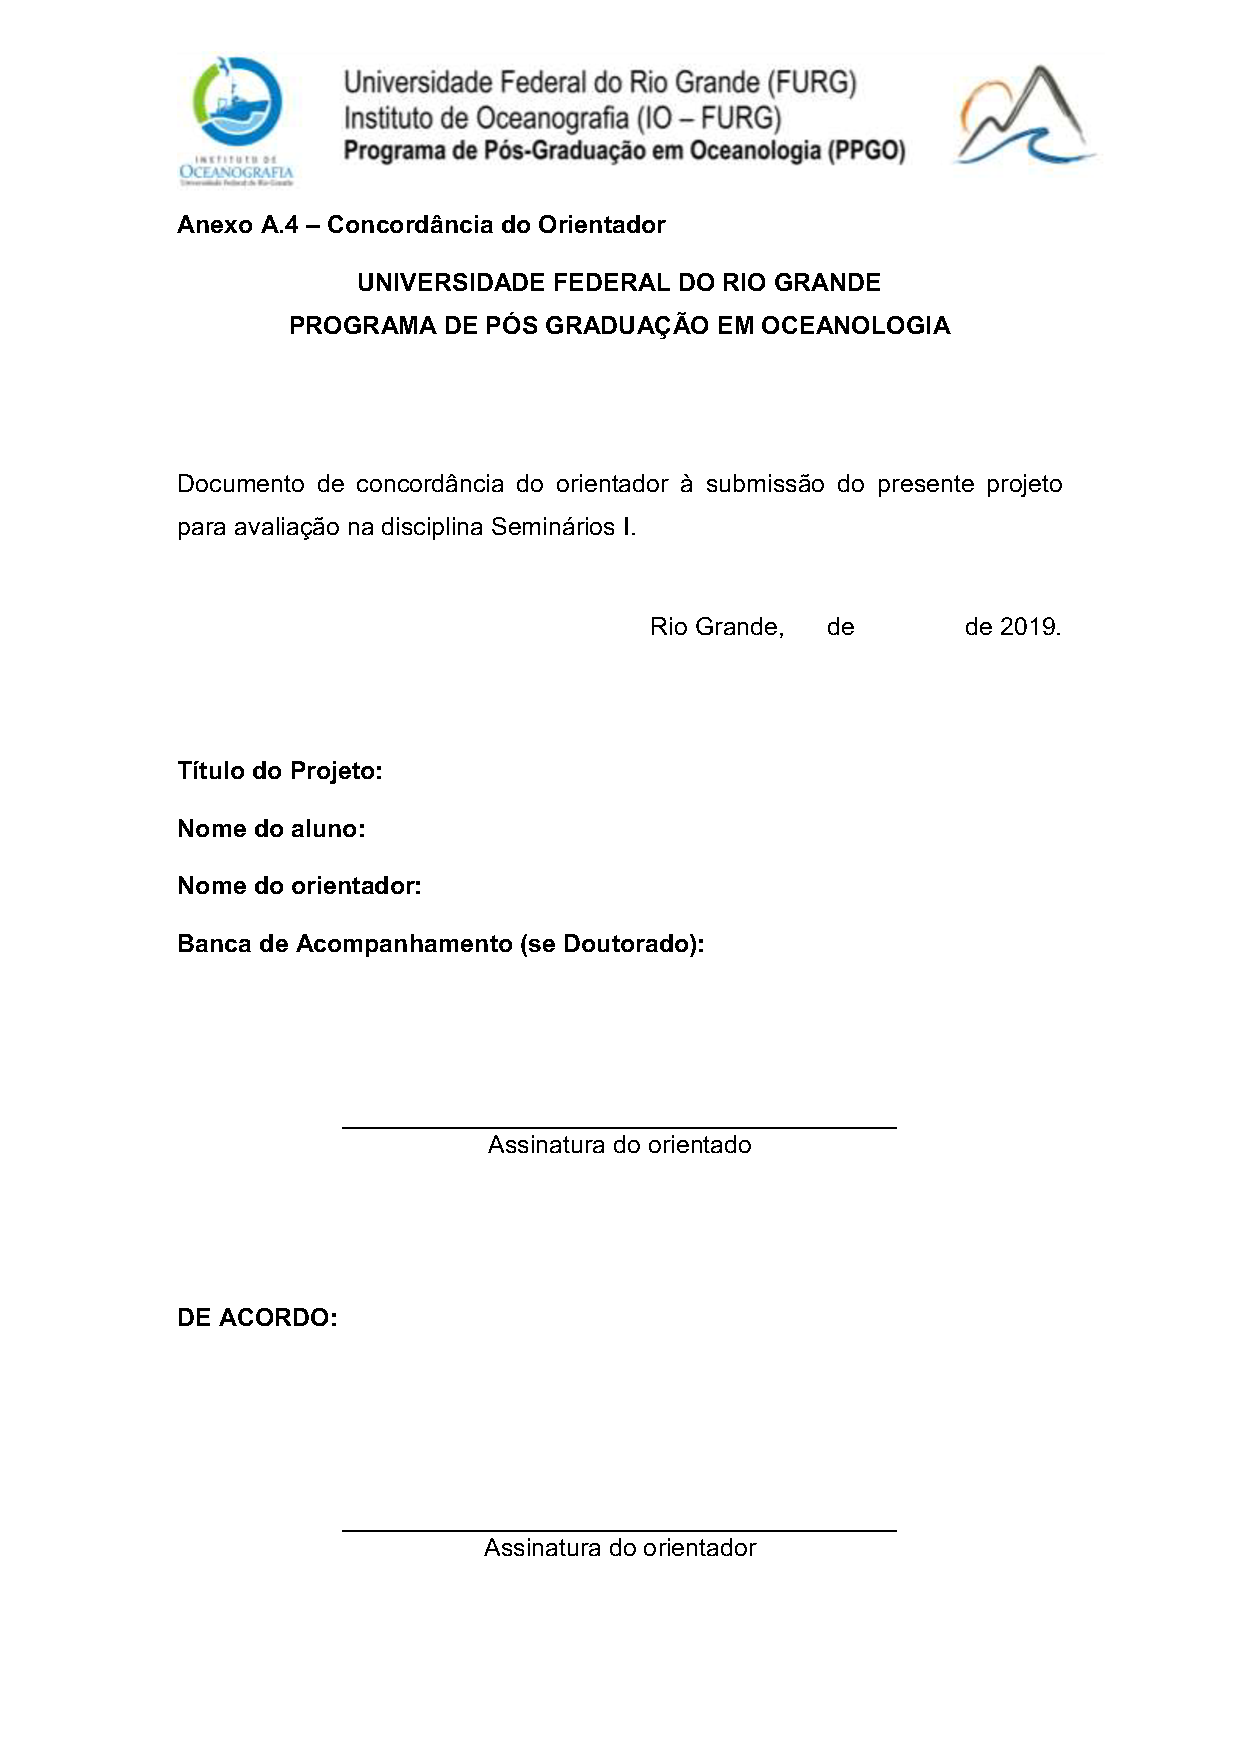
\includepdf[pages={1}]{../Anexo5_NORMAS_DAS_DISCIPLINAS_DE_SEMINRIOS.pdf}
\end{document}